% =======================================================================================
\section{Results}
\label{app:results}\label{app:results-narrow}\label{app:results-full}
% =======================================================================================
% Numbers: scripts/numbers_results.py -> numbers/results.tex; figure: scripts/fig_results.py.
% Input: data/runs/source-count.json (local), from scripts/import_runs.py over outputs/runs/261103-*.

The results are those of six runs that differ only in the band and in the number of sources per
window: $S={}$\ResultsNarrowCounts{} on the narrow band,
\qtyrange{\ResultsNarrowLowMhz}{\ResultsNarrowHighMhz}{\milli\hertz}, and $S={}$\ResultsFullCounts{} on the
full band, \qtyrange{\ResultsFullLowMhz}{\ResultsFullHighMhz}{\milli\hertz}. Every run uses the B network
(\cref{app:network}), the recipe of \cref{app:training} and the priors of \cref{app:priors}, all at one
commit of the code (\texttt{\ResultsCommit}). Each is evaluated on its own eval catalogue
(\cref{app:evaluation-injections}), \EvaluationInjections{} windows log-uniform over its band, against the
joint chains of the same injections and noise (\cref{app:mcmc}). Widths are $1.4826\,\MAD$ of the draws,
after relabelling to the truth and folding $(\psi,\phi_0)$ (\cref{app:evaluation-matching}), as the flow
over the chains, median over the sources of a band of source \ac{snr}.

\subsection{The Runs}
\label{app:results-runs}

\begin{table}[h]
\centering
\caption{The six runs. Steps and warmup are set per run from the epoch time of a
\qty{30}{\minute} smoke test, so that each run has \ResultsEpochs{} epochs; the hours are those epochs
at the smoke test's A100 step time, without restarts. A cooldown over the last
\qty{\ResultsCooldownPercent}{\percent} closes each run. The last column is the lowest eval-catalog
negative log-likelihood, frame plus flow (\cref{app:training-loop}), and its epoch.}
\label{tab:results-runs}
\small
\begin{tabular}{@{}lrrrrrll@{}}
\toprule
band & $S$ & steps [M] & epochs & warmup & hours & outcome & best NLL (epoch) \\
\midrule
\ResultsRunsRows
\bottomrule
\end{tabular}
\end{table}

\Cref{tab:results-runs} lists the runs. The narrow band ran its three source counts one after the
other on one GPU, and the full band on another; a third GPU cooled down forks from each run's
snapshots and evaluated every finished run and fork (\cref{app:training-loop}). Four runs trained to
their end with every loss finite. The full-band run with $S=4$ diverged at epoch
\ResultsFullFourDivergedEpoch, just before its cooldown, after isolated single-step spikes of the
frame's loss (\cref{app:training-optimiser}); it is evaluated at its best checkpoint, epoch
\ResultsFullFourBestEpoch, which never cooled down, and its fork from epoch 32 stands for it below.
\textcolor{red}{TODO(run): the full band with $S=16$ is training until about 11 November; its row,
forks and comparison follow.}

\subsection{Widths Against the Joint \acs{mcmc}}
\label{app:results-mcmc}

\begin{table*}[t]
\centering
\caption{Flow over joint-\ac{mcmc} width per parameter, median over the sources of each band of
source \ac{snr} ($n$ sources), for the model of each band and source count with the lowest eval-catalog
loss among the main run and its four cooldown forks (\cref{tab:results-forks}). Found: share of the
sources with an $f_0$ width below one bin. Coverage: share of true flow coordinates inside the
central \qty{68}{\percent} and \qty{95}{\percent} intervals, over the eight coordinates and the sources
of the band, after relabelling to the truth (optimistic, \cref{app:evaluation-matching}). $\alpha$ and
$\delta$ are equatorial. Below $\snr=7$ (not shown) the ratios are
\ResultsFaintWidthLo--\ResultsFaintWidthHi{} for every parameter and model but narrow $S=8$, whose $f_0$
ratio is \ResultsNarrowEightFaintFzero.}
\label{tab:results-widths}
\small
\begin{tabular}{@{}llrrrrrrrrrr@{}}
\toprule
model & \acs{snr} & $n$ & $f_0$ & $\log\fdot$ & $\log\Amp$ & $\alpha$ & $\delta$ & $\sin\iota$ & found & \multicolumn{2}{c}{coverage 68 / 95} \\
\midrule
\ResultsWidthRows
\bottomrule
\end{tabular}
\end{table*}

\begin{figure*}[t]
\centering
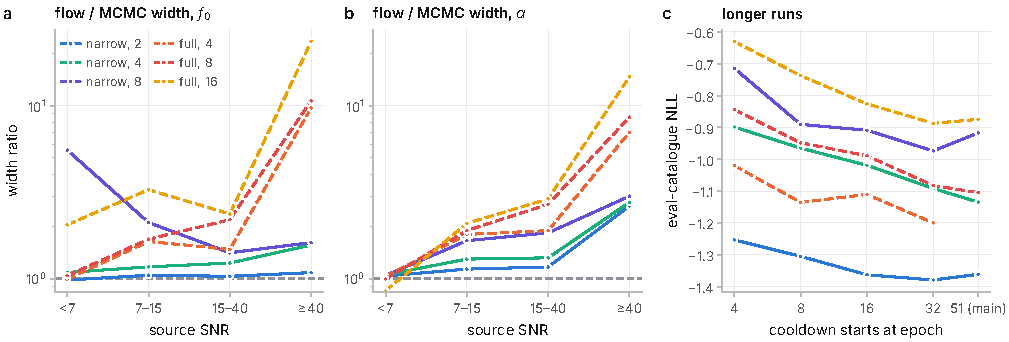
\includegraphics[width=\textwidth]{figures/results.pdf}
\caption{(a), (b)~Flow over joint-\ac{mcmc} width of $f_0$ and of the right ascension against the
source \ac{snr}, for the models of \cref{tab:results-widths}; narrow band solid, full band dashed. (c)~The
eval-catalog loss of the cooldown forks against the epoch at which their cooldown starts, and of the
main runs at theirs; the full band with $S=4$ has no cooled main run.}
\label{fig:results}
\end{figure*}

\paragraph{Faint sources.}
Below $\snr=7$ the target is close to the prior, and the flow returns it: every width is within a few
per cent of the chains' (\cref{tab:results-widths}). The exception is the narrow band with $S=8$, whose
faint sources come out \ResultsNarrowEightFaintFzero{} times wider in $f_0$ than the chains'. A likely cause, not yet checked, is that with eight sources in
\PriorsNarrowW{} bins faint neighbours overlap within their prior widths, where the frequency order of
the slots no longer tells them apart.

\paragraph{The narrow band.}
With two sources per window the flow matches the chains: at $\snr=7$--40 every width ratio is
\ResultsNarrowTwoWidthLo--\ResultsNarrowTwoWidthHi, $f_0$ \ResultsNarrowTwoFzeroMid{} at
$\snr=15$--40 (\cref{fig:results}a). It finds \qty{\ResultsNarrowTwoFoundLow}{\percent} of the
sources at $\snr=7$--15, and of the $f_0$ draws of sources at $\snr\ge15$,
\qty{\ResultsNarrowTwoOff}{\percent} fall off the chains' peak (more than five chain widths, and half a
bin, from its median), against \qty{\ResultsNarrowTwoMcmcOff}{\percent} of the chains' own draws. Each
doubling of $S$ widens the posteriors and fattens their tails. With four sources $f_0$ is
\ResultsNarrowFourFzeroLo--\ResultsNarrowFourFzeroHi{} times the chains' width at $\snr=7$--40 and the
right ascension \ResultsNarrowFourSkyMid{} times at $\snr=15$--40; \qty{\ResultsNarrowFourFoundLow}{\percent}
are found at $\snr=7$--15, and \qty{\ResultsNarrowFourOff}{\percent} of the loud sources' draws are off
the peak (chains: \qty{\ResultsNarrowFourMcmcOff}{\percent}). With eight, $f_0$ is
\ResultsNarrowEightFzeroLow{} times the chains' width at $\snr=7$--15 and \ResultsNarrowEightFzeroMid{} at
15--40, \qty{\ResultsNarrowEightFoundLow}{\percent} are found at $\snr=7$--15, and
\qty{\ResultsNarrowEightOff}{\percent} of the loud draws are off the peak, against
\qty{\ResultsNarrowEightMcmcOff}{\percent} of the chains'. The sky widens at every $S$ and grows with the
\ac{snr}, to two to three times the chains' above $\snr=40$ (\cref{fig:results}b), where the narrow
band has only a handful of sources.

\paragraph{The full band.}
On the full band the flow is close to the chains only for faint sources. At $\snr=15$--40 its $f_0$
widths are \ResultsFullFourFzeroMid{} ($S=4$) and \ResultsFullEightFzeroMid{} ($S=8$) times the chains',
and above $\snr=40$ they are \ResultsFullFourFzeroLoud{} and \ResultsFullEightFzeroLoud{} times, with
$\log\fdot$ \ResultsFullFourFdotLoud{} and \ResultsFullEightFdotLoud{} times and the right ascension
\ResultsFullFourSkyLoud{} and \ResultsFullEightSkyLoud{} times; amplitude and inclination stay within
\ResultsFullFourAmpLoud{} and \ResultsFullEightAmpLoud. Only \qty{\ResultsFullFourFoundLoud}{\percent} and
\qty{\ResultsFullEightFoundLoud}{\percent} of the loud sources are found, and
\qty{\ResultsFullFourOff}{\percent} and \qty{\ResultsFullEightOff}{\percent} of their draws fall off the
chains' peak, against \qty{\ResultsFullFourMcmcOff}{\percent} and \qty{\ResultsFullEightMcmcOff}{\percent}
of the chains' own. The loud sources of the full band are those whose posteriors are narrowest against
the prior and whose responses span the most bins (\cref{app:forward-model}), the regime the per-source
frame is meant for (\cref{app:fm-sensitivity}); the full-band models do not resolve them yet. \textcolor{red}{TODO(analysis): where in frequency the unfound loud
sources sit (most above \qty{10}{\milli\hertz} in a first look at full $S=4$), and whether the frame or
the flow is the wide part.}

\paragraph{Calibration.}
Every eval, main runs and forks, \ResultsEvals{} in all, covers
\ResultsCoverSixtyEightLo--\ResultsCoverSixtyEightHi{} of the true coordinates at the
\qty{68}{\percent} level and \ResultsCoverNinetyFiveLo--\ResultsCoverNinetyFiveHi{} at
\qty{95}{\percent}, pooled over coordinates and sources, including the full-band models that are an
order of magnitude too wide on loud sources. As the mocks predicted (\cref{app:evaluation-mocks}),
coverage after relabelling does not see excess width: only the comparison with the chains does.
\textcolor{red}{TODO(runs): rank tests, \acs{tarp} and proper scores of the validation pass, which never
sees the truth, once the scorecards are back.}

\subsection{Longer Runs}
\label{app:results-forks}

\begin{table}[h]
\centering
\caption{Eval-catalog loss / flow over joint-\ac{mcmc} $f_0$ width at $\snr=15$--40, for the forks that
start their cooldown at epochs 4 to 32, and for the main run, which starts it at the planned
\qty{80}{\percent} of its \ResultsEpochs{} epochs (full $S=4$: its best, uncooled, checkpoint).}
\label{tab:results-forks}
\small
\begin{tabular}{@{}lccccc@{}}
\toprule
 & e4 & e8 & e16 & e32 & main \\
\midrule
\ResultsForkRows
\bottomrule
\end{tabular}
\end{table}

The forks give the same configuration trained for 5, 10, 20 and 40 epochs (\cref{app:training-loop}).
Their eval-catalog loss falls with the training length (\cref{tab:results-forks}, \cref{fig:results}c):
by \ResultsNarrowTwoForkGain{} nats from epoch 4 to 32 on the narrow band with $S=2$ and by
\ResultsFullFourForkGain{} on the full band with $S=4$, and the $f_0$ widths shrink toward the chains'
with it. The cooldown matters most on the full band: the diverged full-band run with $S=4$, never cooled,
has loud $f_0$ widths \ResultsFullFourMainLoud{} times the chains', against \ResultsFullFourForkLoud{}
for its fork from epoch 32. Beyond epoch 32 the main runs gain on two configurations and lose on two
(\cref{app:training-schedules}); with one seed per configuration, differences of a few hundredths of a
nat are within the run-to-run spread we have not measured.

\subsection{Not Yet Run}
\label{app:results-pending}

\begin{itemize}
  \item \textcolor{red}{TODO(runs): full band, $S=16$: row, forks, widths.}
  \item \textcolor{red}{TODO(runs): validation table, $\gamma$ $p$-values and energy scores per test
    quantity; rank \acs{ecdf} minus uniform with the simultaneous band.}
  \item \textcolor{red}{TODO(runs): sampler steps at which the widths settle (\cref{app:evaluation-sampler})
    and the robustness probes.}
  \item \textcolor{red}{TODO(figure): corner plot of flow, joint \acs{mcmc} and Fisher draws on one
    crowded eval window, from the runs' corner pages.}
\end{itemize}
